\chapter{Alignment in sung music}
\label{chap:alignment_in_sung_music}

%\lettrine{I}{introduction} to this chapter\ldots

%\pagebreak

\section{abstract}
\label{sec:abstract}

\section{Introduction}
\label{sec:introduction}

The rhetorical aspects of music and spoken language can be described in musical terms.
Melody, pitch, timbre, rhythm and tempo are all common in description of music, as they are in speech \citep{Molino2000toward, Jackendoff2009parallels}.
Some spoken language related phenomena can also be described using musical means \citep[as in][]{Day2013speech}.

In this paper, we investigate a speech-related phenomenon, namely \emph{phonetic convergence}, in sung music.
Phonetic convergence is a process in which interlocutors become more similar to each other in terms of phonetic features while interacting \citep{Pardo2006phonetic, Kim2011phonetic}.
Methods commonly utilized in this research topic were adapted to suit musical material to examine whether convergence can be found also in singing and whether the musical nature of the used materials can shed light on additional aspects of convergence.

The two types of vocal capabilities, singing and speech, share some properties in both production and perception.
Such common properties include articulation rate, intensity, timbre, and others.
Another important aspect is that both have a temporal dimension and evolve over time.
However, music consists of defined \emph{absolute} pitch and rhythmic targets.
This is even more salient when dealing with an already known musical material, as both the singer and the listener already have expectations regarding the tones before they are produced \citep{Meyer2008emotion}.
In speech, on the other hand, the phonetic features of a specific utterance are not expected to match specific absolute values.

\begin{snippet}[t]
	\centering
	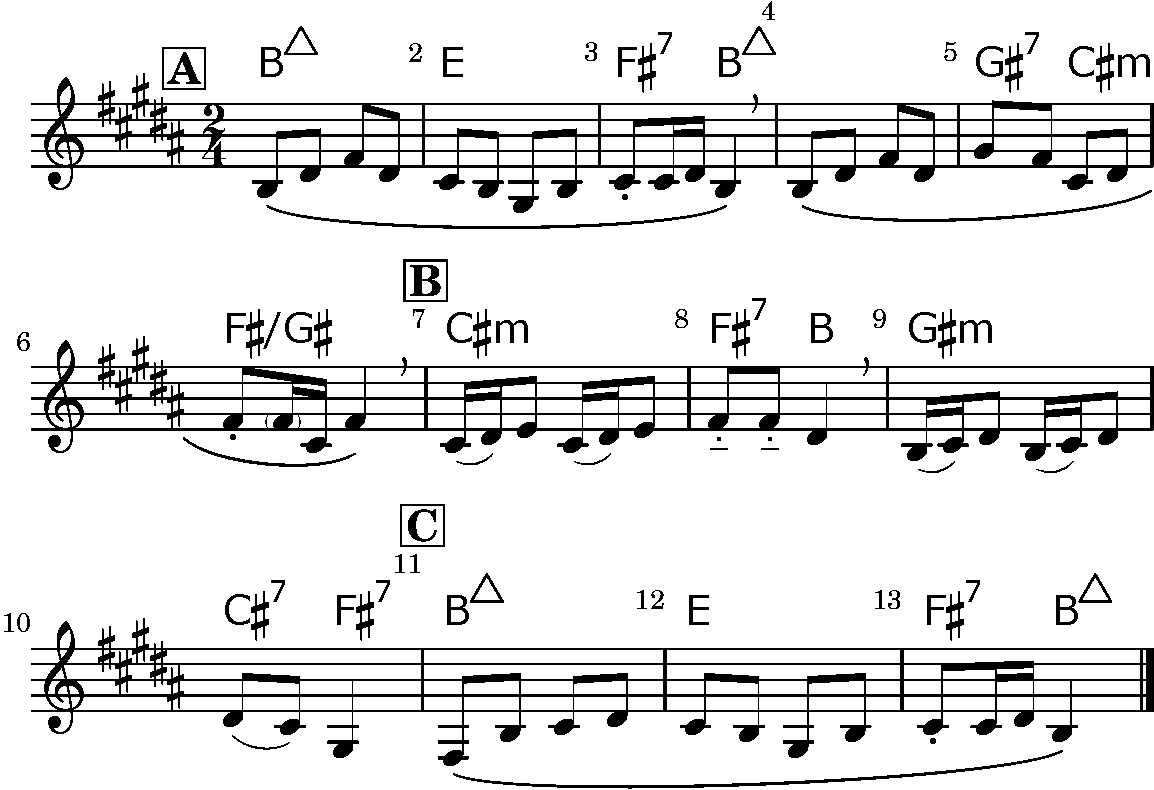
\includegraphics[width=\linewidth]{yakinton}
	\caption{The Yakinton lullaby transposed to B major.
		The square labels \enquote{A}, \enquote{B}, and \enquote{C} mark the \emph{theme}, \emph{bridge} (or \emph{development}), and \emph{recapitulation} sections of the song.
		The breath marks are placed where the participants are expected to make a brief break and/or lengthen the ending of a phrase.
		The first sixteenth note in bar six is in brackets since it is not present in the original melody and was therefore also excluded in the recorded version played to the participants.
		However, it is common to add it, and indeed all participants included it in both performances.}
	\label{snippet:yakinton}
	\addcontentsline{lof}{section}{Snippet: Yakinton lullaby}
\end{snippet}

Phonetic convergence has been studied with respect to various prosodic features, such as speech rate \citep{Schweitzer2013convergence, Pardo2012phonetic}, fundamental frequency \citep{Babel2012role, Collins1998convergence}, intonation \citep{DImperio2014phonetic, Simonet2011intonational}, rhythm \citep{Krivokapic2013rhythm}, and more.
Due to similarities and dissimilarities between speech and music, we believe it can be rewarding to see whether convergence can be found in singing as well, and whether it operates differently.
As both speaking and singing are used in social contexts, external factors may potentially affect them.
In the case of music, convergence can be expressed in different aspects than in speech, e.g., singing the notes more accurately, shifting the musical key, adapting to a different tempo, etc.
Furthermore, seeing that the tonal targets in singing are pre-defined, there are precise targets for production -- either from a heard example or from one's mental memory -- in an experimental setting.
Therefore, the participants' productions can be directly compared with some \enquote{ground truth}.

The main research question of this work is whether convergence occurs in singing as well, and, if so, whether specific parts of the musical piece are prone to undergo changes.
Our hypothesis is that convergence will be found in the participants' performances with respect to the pre-recorded stimuli.
This can be realized on the absolute level, meaning that the participants shift their overall pitch range (i.e., the \emph{key}) and tempo to be closer to the recording, or relative to their own singing by making the pitch and temporal intervals between the target notes more accurate.
An additional question is how the familiarity with the musical material affects reproduction.
The expectation here is that the participants' performances of the familiar song will be accurate even before listening to a version of it in terms of deviation from the target intervals, but even more so after listening.
When reproducing an unfamiliar melody, it is not expected that the participant will remember it in its entirety, but rather that they would stick to repeating segments or parts with smaller intervals and simpler rhythms.

% structure of paper (short version)
%The methods and materials are described in \cref{sec:method}.
%\cref{sec:analysis} comprises the applied analyses, followed by the results presented in \cref{sec:results}.
%Finally, interpretations and additional observations are discussed in \cref{sec:discussion_and_conclusion}, which also concludes the paper.

The present study consists of two shadowing experiments \citep[cf.][]{Goldinger1998echoes}.
Sung lullabies were chosen in this work, as they are presumably more memorable than other musical genres and than instrumental pieces \citep{Weiss2012something, Trehub1991music}.
Shadowing -- here, delayed, non-immediate shadowing -- is a common methodology in convergence studies \cite[e.g.,][]{Pardo2018comparison}.
The first experiment tests convergence effects between two performances of the participants, one before and one after listening to a pre-recorded version of a song \emph{familiar} to them.
In the second experiment, participants listened to another, \emph{unfamiliar} song and replicated it to their best ability.
This experiment tests which prosodic features would be replicated best when it is not likely that the participants would remember all aspects of the musical material.
The experimental procedures and materials are described in \cref{sec:method}.
\cref{sec:analysis} presents the methods applied to analyze the prosodic properties \emph{pitch}, \emph{tempo}, and \emph{rhythm}.
%These are the two main features that are directly noted in musical sheets, and play an important role in both speech and music and have been studied in speech convergence studies \citep{Schweitzer2013convergence}.
Results are presented in \cref{sec:results}, along with some representative examples from the participants' performances.
Finally, interpretations and additional observations are discussed in \cref{sec:discussion_and_conclusion}, which also concludes the paper.

\section{Method}
\label{sec:method}

\subsection{Material}
\label{subsec:material}

\begin{snippet}[t]
	\centering
	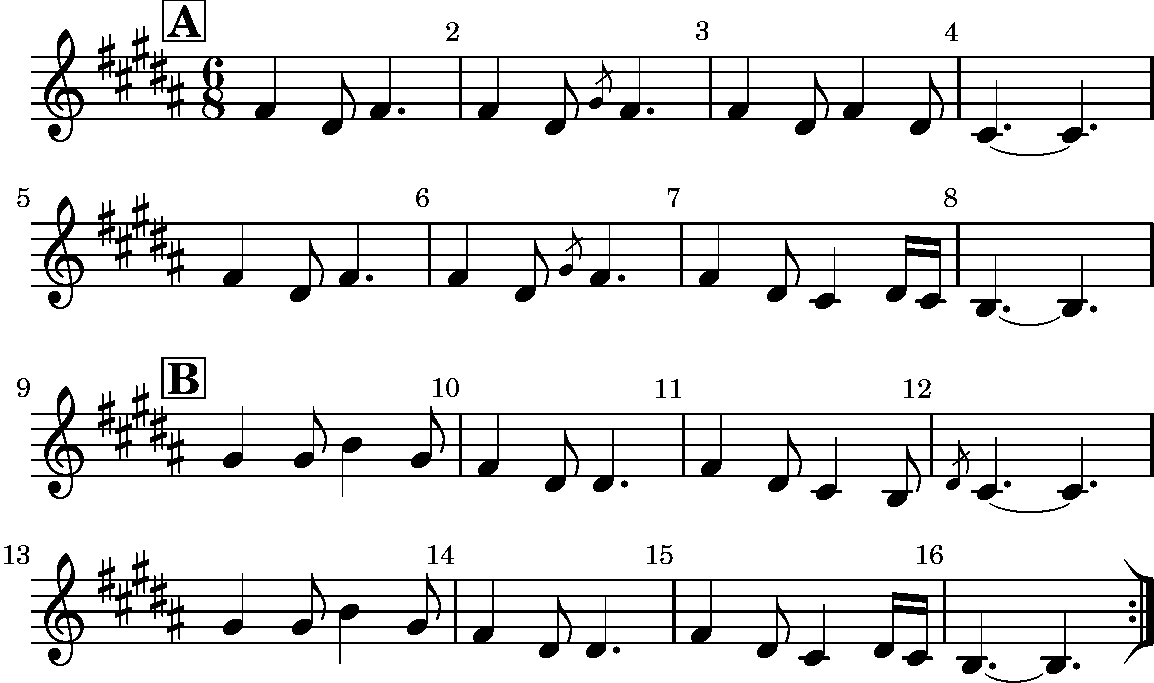
\includegraphics[width=\linewidth]{lullaby}
	\caption{Neutral lullaby.
			 The square labels \enquote{A} and \enquote{B} mark the structural parts.
		 	 The grace notes in bars 2, 6, and 12 were included in the recording but due to their secondary melodic role did not penalize performances that lacked them.}
	\label{snippet:uni-lullaby}
	\addcontentsline{lof}{section}{Snippet: Universal lullaby}
\end{snippet}

Two lullabies were used in the experiment: The first is \enquote{Tune for the Yakinton}\footnote{Pizmon LaYakinton%
%	(\emph{Hebrew:}\hebrewtext{פזמון ליקינטון})
, written by Leah Goldberg in 1940. \emph{Yakinton} is the Hebrew name of the Hyacinth plant.} (hereafter \enquote{Yakinton}, see \cref{snippet:yakinton}), which is a famous Israeli children song.
The second is a neutral lullaby composed for experimental purposes \citep[][pp.~22-47, see \cref{snippet:uni-lullaby}]{Twig2016universal}, which contains \emph{cross-cultural similarities} such as repetitiveness, simple melody, and a limited inventory of tonal and rhythmic elements \citep{Unyk1992lullabies, Trehub1993maternal}.
Therefore, while the first one is assumed to be known to the participants, they could not be familiar with the second one.
Both lullabies are short (13 bars at \musQuarter~=~61 ($\approx$\SI{26.5}{\second}) and 16 bars at \musQuarterDotted~=~33 ($\approx$\SI{58}{\second}), respectively) and in major keys.
Both songs were recorded a cappella by a trained female singer in the same age group as the participants in a professional recording studio at \SI{44.1}{\kilo\hertz} sampling rate and 16~bit resolution.
To avoid changes in voice production, decrease vibrato, and limit the singing effort, the songs were transposed and recorded in B major, which is relatively low for female voices.
This also avoids influences originating from the use of different keys.
The syllable \textipa{[na]} was used throughout the songs in both the recordings and participants' productions to eliminate any bias due to their lyrics (see \cref{subsec:procedure}).
This way, the possibility that the participants would know the melodies but not the lyrics was avoided as well.

\subsection{Participants}
\label{subsec:participants}

Six participants, all of which are mothers with no hearing impairments to recently born babies, took part in the experiments.
Their age ranged from 29 to 37 years (mean 35.5 $\pm$3.25) and the age of their babies ranged from one to seven months (mean 4.5 $\pm$3.5).
For three of the mothers this was the first child.
To further homogenize the participants' characteristics, their musical education and experience was controlled as well.
None had any professional-level musical background, while four disclosed they have been playing an instrument or singing.

In the pre-verbal phase, parents often sing to their babies.
When communicating with infants, adults tend to use exaggerated prosody with elevated melodic pitch and distinct rhythmic patterns \citep{Fernald1991prosody}.
The increased use of singing as well as its function as a means of communication with their babies \citep[see][]{Street2003mothers,Papouvsek1991meanings} made mothers of small babies suitable for this experiment.
Since the participants' singing capabilities are essential for their performance in the experiment, it was also confirmed that they regularly sing lullabies for their babies.
Furthermore, as we are dealing with a specific lullaby (see \cref{subsec:material}), their familiarity with it was also considered.
All the participants reported that they know the familiar lullaby well enough to spontaneously sing it (as described in \cref{subsec:procedure}).

\subsection{Procedure}
\label{subsec:procedure}

The experiment comprised two shadowing experiments, one for each song, which were carried out consecutively.

In the first experiment, the participants were first asked to sing the Yakinton's melody with the syllable \textipa{[na]} instead of its lyrics.
Beside that, no specific instructions were given, e.g., regarding the tempo, the key, or any other musical preference.
Subsequently, the participants listened to the pre-recorded version of the song (see \cref{subsec:material}) via wired over-ear headphones (Phillips SHL3060).
Following that, they sung the song once more and answered some questions regarding the recorded version of the song, to determine how much it differs from the one in their mental memory.
Importantly, no reference to either their previous production or the recorded version was made by using wordings like \enquote{repeat}, \enquote{mimic}, \enquote{like before}, etc.

The second experiment comprised only a shadowing performance, as the participants were intentionally unfamiliar with the neutral lullaby.
After listening to the pre-recorded version of the lullaby, they were instructed to sing it themselves.
This required not only their singing capabilities, but also their musical memory.
As explained in \cref{subsec:material}, this song was specifically composed with common characteristics of the genre in mind and should therefore contain similar melodic and harmonic contents to the song in the first experiment.

%In addition to the short questions in the first experiment, the participants also answered a personal questionnaire before starting the experiment and a closing questionnaire at the end.
%The whole procedure lasted about \SI{15}{\minute} in total per participant.

\section{Analysis}
\label{sec:analysis}

\begin{figure}[t]
	\centering
	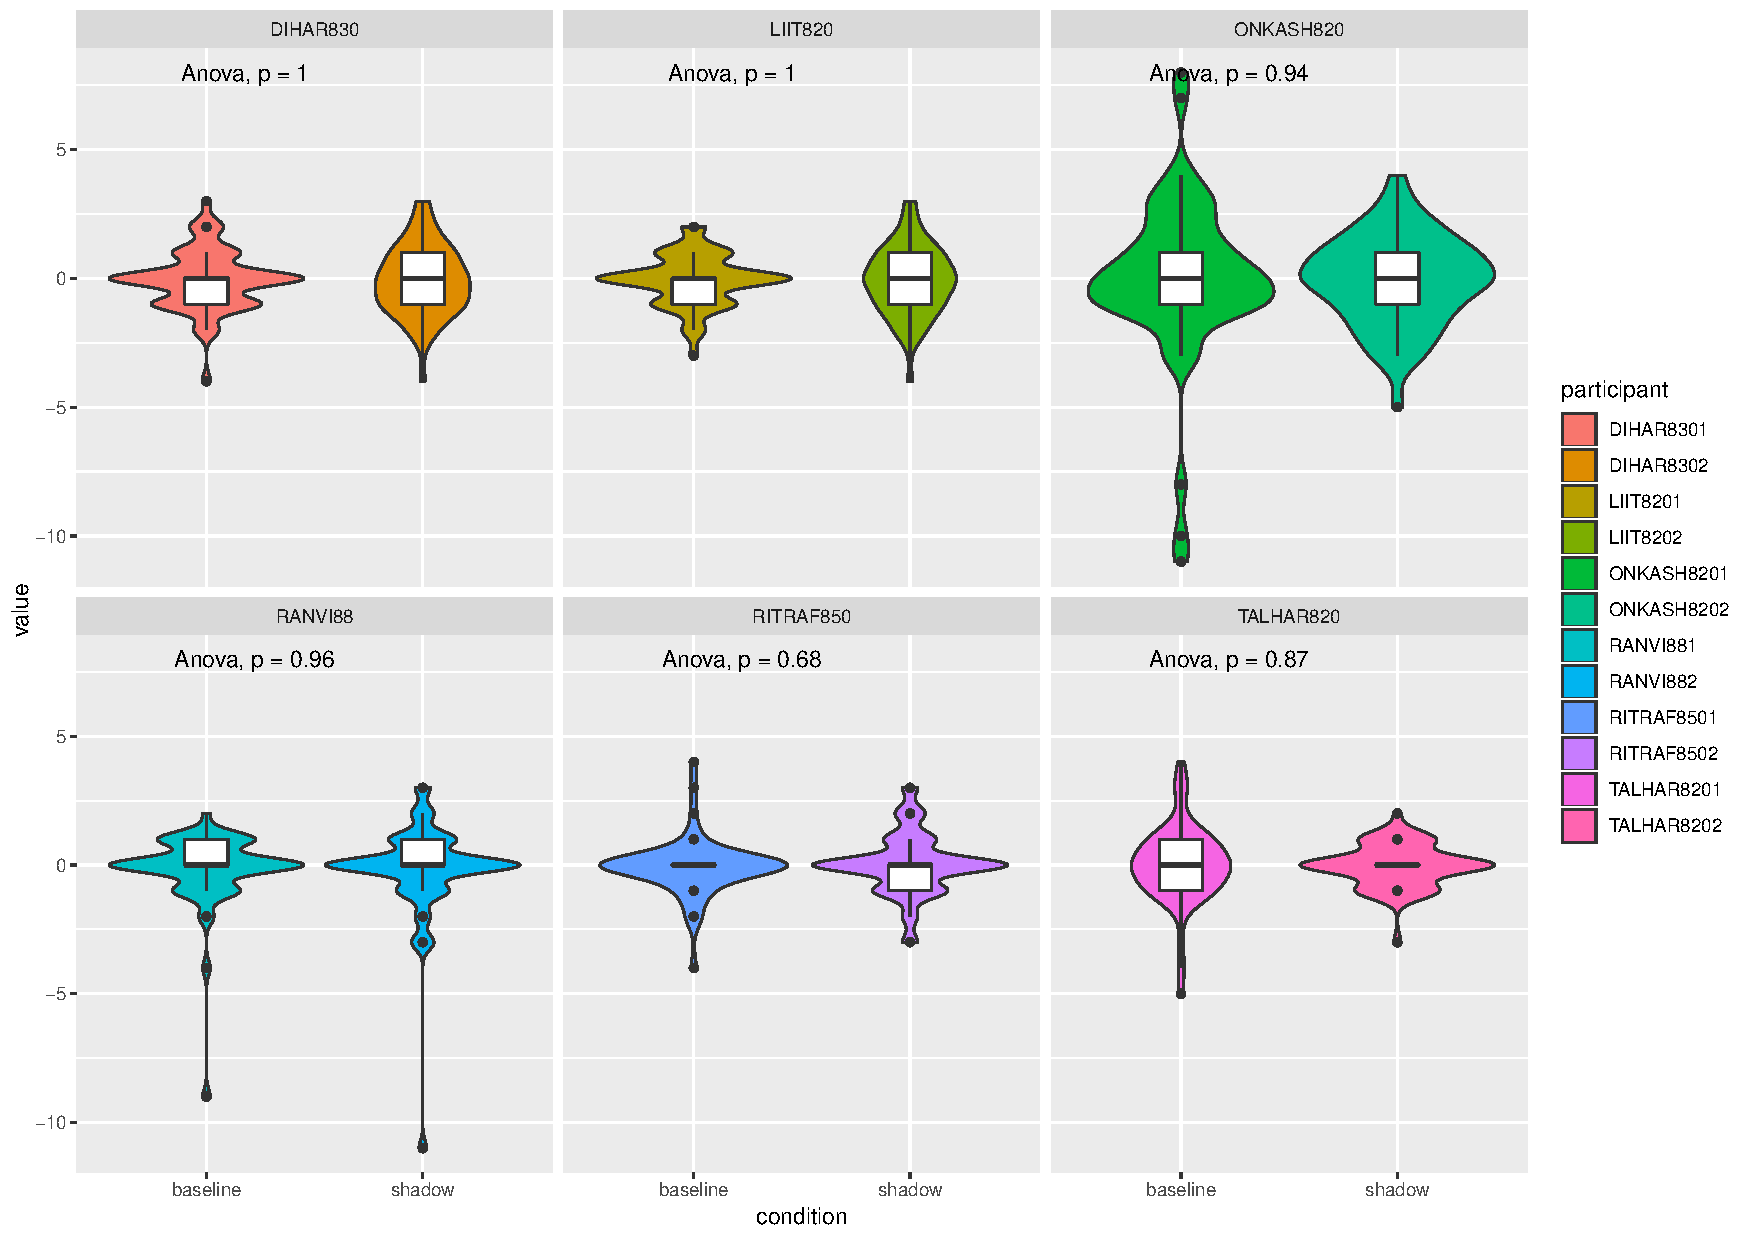
\includegraphics[width=\linewidth]{violin_facet_dev}
	\caption[Summary of within-participant interval deviation distribution]
		{Comparison between the distribution of deviations from the correct intervals in baseline (red) and shadowing (blue) performances.
		The numbers on the x-axis are the number of \acp{qt} above or below the correct interval.}
	\label{fig:violin_facet_dev}
	\todo[inline]{refer to this figure in text (was not in original paper)}
\end{figure}

\begin{figure}[t]
	\centering
	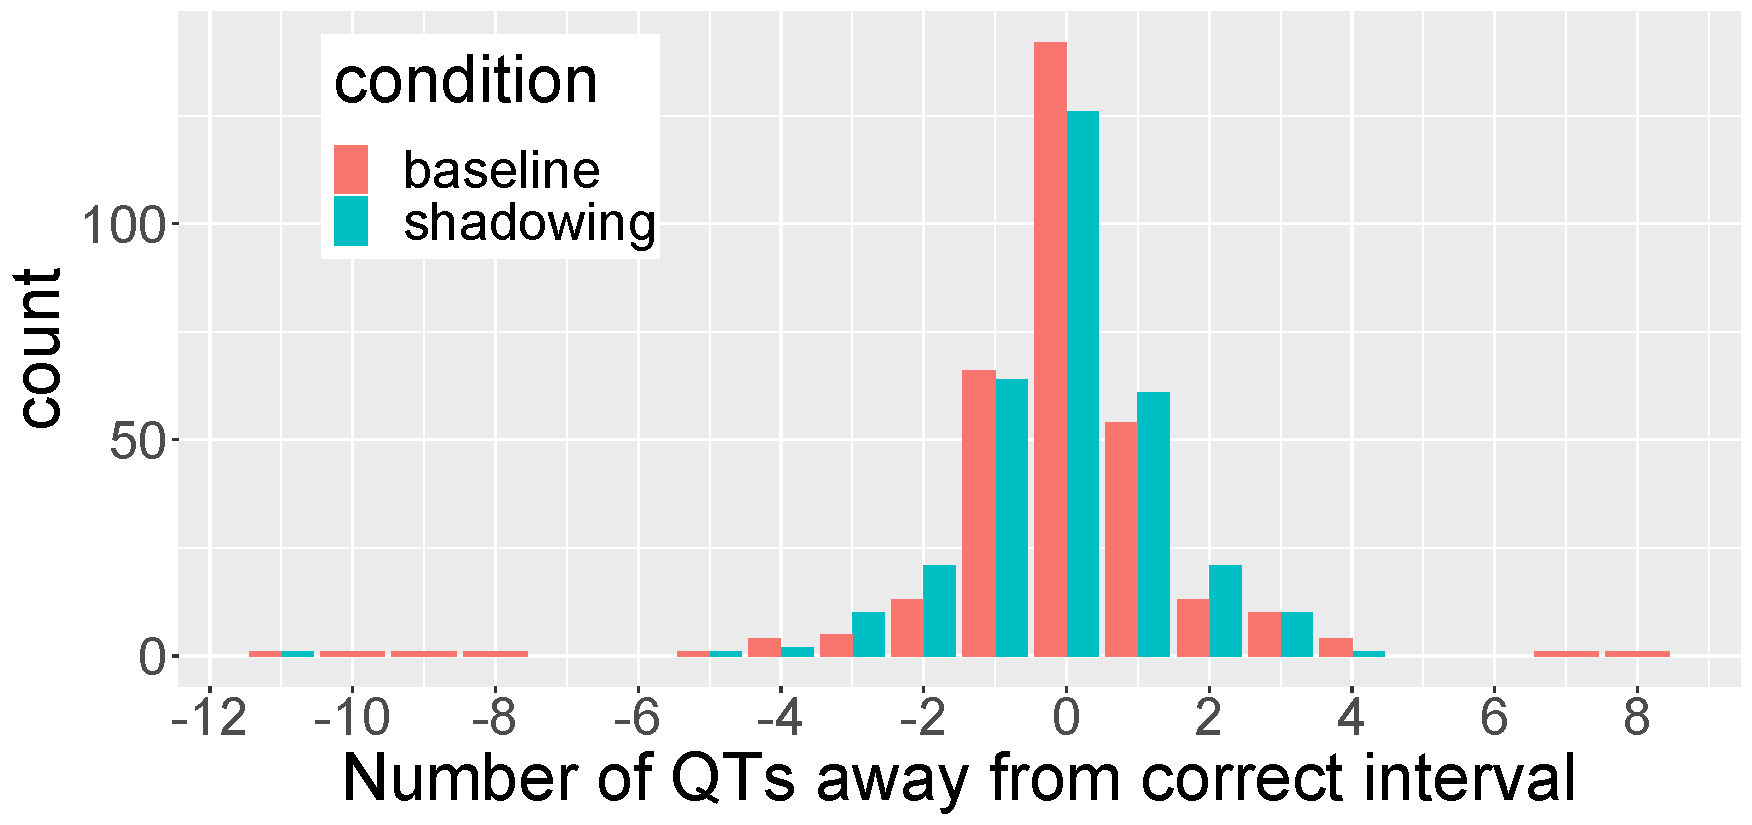
\includegraphics[width=\linewidth]{barplot_QT_distances}
	\caption[Distribution of interval deviations]
	{Comparison between the distribution of deviations from the correct intervals in baseline (red) and shadowing (blue) performances.
		The numbers on the x-axis are the number of \acp{qt} above or below the correct interval.}
	\label{fig:barplot_QT_distances}
\end{figure}

Since the participants aimed to produce specific musical notes (as opposed to non-specific absolute frequency while speaking), tones were used for measuring pitch instead of raw \si{\hertz} values.
To increase the pitch resolution, quarter tones (\acp{qt}) were used instead of semitones.
This enables a more fine-grade analysis, which can capture more subtle off-key singing to differentiate the performances better.
%The performances were manually transcribed in Sibelius 6
%\todo{version footnote}
%and were verified using the corresponding MIDI output against the recordings.
Furthermore, segmentation of the performance into individual tones was done manually.
Silences, non-singing, breaths between phrases, etc.\ were segmented as well.
The tone frequencies were determined by the median of the measured frequencies during this tone's duration, excluding the first and last \SI{10}{\percent} of the tone duration.
This excludes transitions between tones and smooths out vibrato and \textit{ad lib} ornaments.
These values were extracted using Praat \citep{Boersma2001praat} and manually verified.
Subsequently, the note assigned to each singing segment was determined by selecting the closest \ac{qt} to the measured frequency in the corresponding segment.
The mapping between tone frequencies and \acp{qt} (relative to middle A) was done using the formula

\begin{equation}
	\label{eq:quarter_tones_formula}
	frequency(QT_n) = 440 \cdot \sqrt[24]{2}^n,
\end{equation}
\eqname{\Acl{qt} frequency calculation (equal temperament)}\noindent
%
where $n$ is the number of \acp{qt} away from the middle A key (cf.\ \citet{DeKlerk1979equal}) and \SI{440}{\hertz} is the frequency of middle A.
This formula is based on the equal temperament.
%, which can be assumed to be the tuning system with which the participants grew up.
QTs are denoted here with the symbols \hspace{-0.18cm}
$\vcenter{\hbox{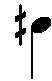
\includegraphics[height=15pt]{qt_c-cih}}}$ and 
$\vcenter{\hbox{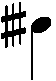
\includegraphics[height=15pt]{qt_c-cisih}}}$ for one \ac{qt} and three \acp{qt} above a note, respectively.
Ultimately, tonal deviations were measured per interval, rather than per tone, as the latter would depend on the key the participants chose, while the former measures tonal accuracy independently of key.

Tempo was measured for an entire performance, taking into account only singing segments (similar to articulation rate in speech).
This ensures that pauses between phrases do not influence the perceived singing tempo, and that occasional, non-scripted lengthenings (e.g., short ritardandos and fermate at the end of phrases) do not mark a specific note as being out of rhythm.
Tempo was measured in \ac{bpm}, which is directly derived from the standard musical notation \musQuarter~=, using the formula

\begin{equation}
	\label{eq:bpm}
	BPM = \frac{N + \delta}{overall\ duration} \cdot 60,
\end{equation}
\eqname{\Acf{bpm}}\noindent
%
where $N$ is the number of beats in the song and $\delta$ is the number of beats added in a specific performance.
Such additions occurred exclusively at the end of phrases (bars 3, 6, 10, and 13 in \cref{snippet:yakinton}), but are not present in the pre-recorded stimulus.
The Yakinton lullaby (\cref{snippet:yakinton}) and the neutral lullaby (\cref{snippet:uni-lullaby}) have 26 quarter beats and 32 dotted quarter beats, respectively.

\section{Results}
\label{sec:results}

As expected, the participants could, for the most part, accurately produce the Yakinton lullaby (\cref{snippet:yakinton}) based merely on their mental representation of it in the baseline phase.
However, as \cref{fig:barplot_QT_distances} shows, these performances included several large deviations of two tones or more, which are not likely to be caused by coincidental imprecise singing.
In the shadowing condition, in comparison, there was only one such large deviation.
This adjustment of obviously wrong tones was apparently driven by the exposure to a correctly sung version.
Other than these corrections, the deviation distributions shown in \cref{fig:barplot_QT_distances} are roughly symmetric and equal to baseline in shadowing conditions.
Surprisingly, the baseline performances had more tones within $\pm1$ \ac{qt} (which for the participants' western ear would still sound correct).
It seems, therefore, that the reference version helped the participants to sing within a more accurate range of tones, but also to show more variation within this range.

The tone-by-tone comparison presented in \cref{fig:barplot_facet_tone_diff} sheds more light on these differences.
It is evident that except for the very first interval, the participants showed greater consecutive variation in the second part of the bridge (label \enquote{B} in \cref{snippet:yakinton}, notes 34 to 42), while in the shadowing condition the first phrase (first seven intervals) show a similar tendency.
Although the bridge moves to a new tonal center, it is not clear why only the second part of it would cause the singers to be less precise.
As for the higher variation at the beginning of the shadowing performances, this points to the process of re-finding the right tones in the participants' key of preference.
This explanation is supported by the key comparisons in \cref{tab:bpm_and_keys}, which show that there was virtually no key change between the baseline and shadowing performances by any of the participants.
Despite that, the unstable beginning of the shadowing performances indicates that listening to the recorded version influenced the participants' tonal accuracy.
They needed about one whole phrase to overcome the influence of the different tonal center in the recorded version and go back to their key of preference.
Interestingly, the only participant who sang in the same key as the recording did change key in the second performance.

\begin{figure}[t]
	\centering
	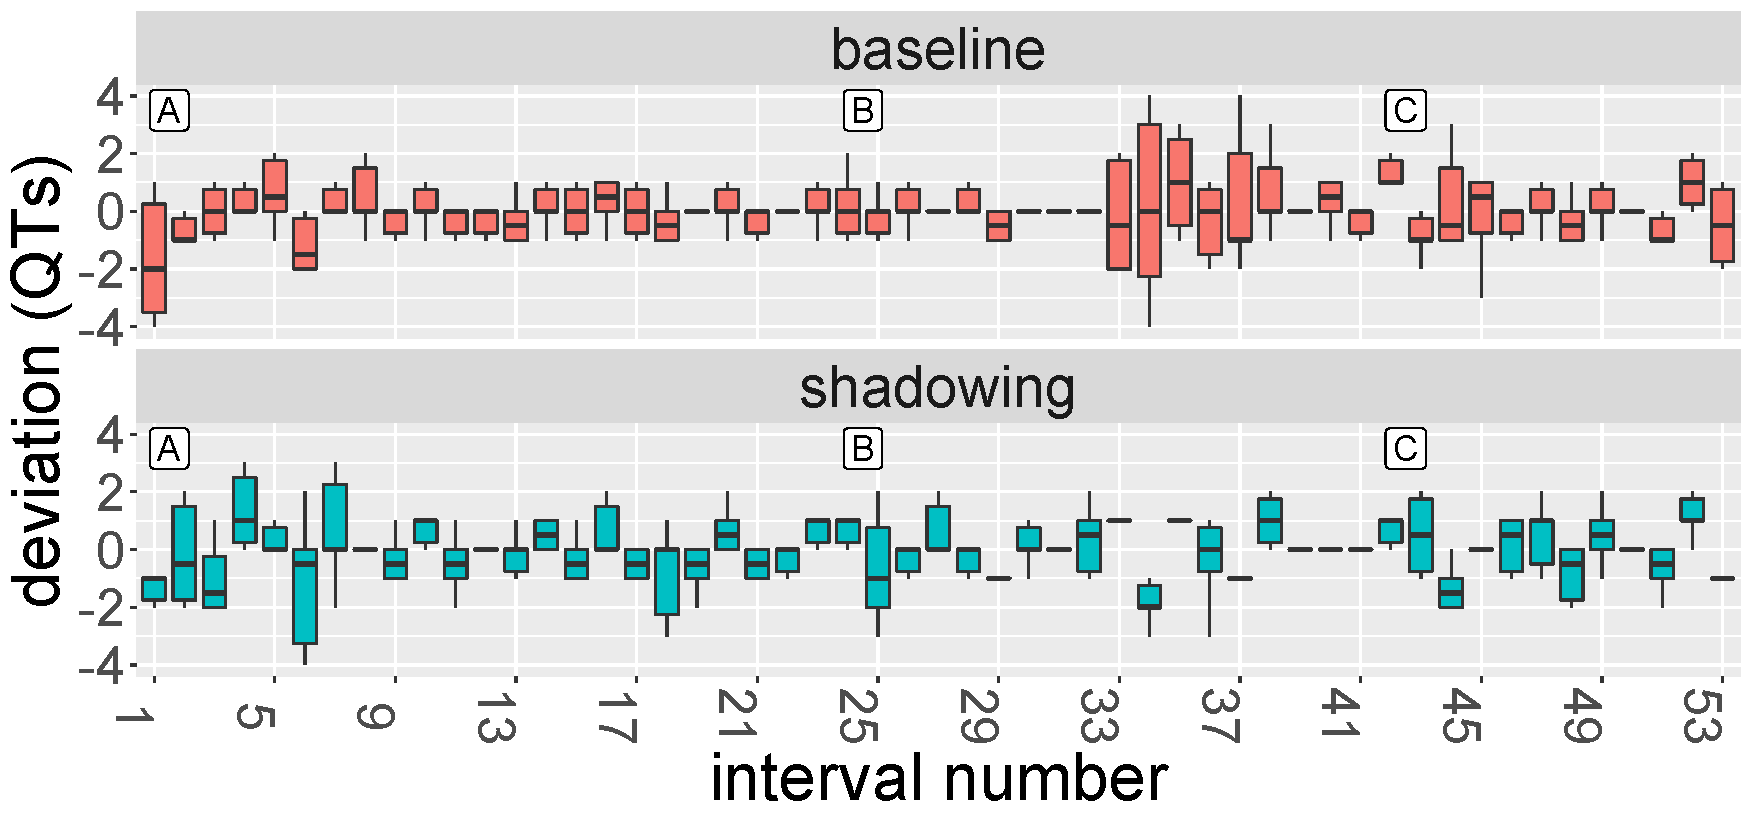
\includegraphics[width=\linewidth]{barplot_facet_tone_diff}
	\caption[Comparison of interval deviation between baseline and shadowing performances]
		{Comparison between the deviation distribution of each interval in baseline (top) and shadowing (bottom) conditions.
		The numbers on the x-axis are the interval indices representing the 53 intervals in the Yakinton lullaby.
		The distances between the intervals sang by the participants and the correct intervals are shown on the y-axis (outliers are omitted).
		The labels \enquote{A}~to~\enquote{C} mark the different parts of the song (and correspond to the same labels in \cref{snippet:yakinton}).}
	\label{fig:barplot_facet_tone_diff}
\end{figure}

The tempo of the recorded version was \SI{61}{\ac{bpm}}.
In the baseline performance, three participants sang faster than that and three more slowly (see \cref{tab:bpm_and_keys}).
All participants changed their tempo so that it was closer to the recorded version.
Moreover, the absolute distance from the recording's tempo decreased in all cases but one.

%\begin{figure*}[t]
%	\centering
%	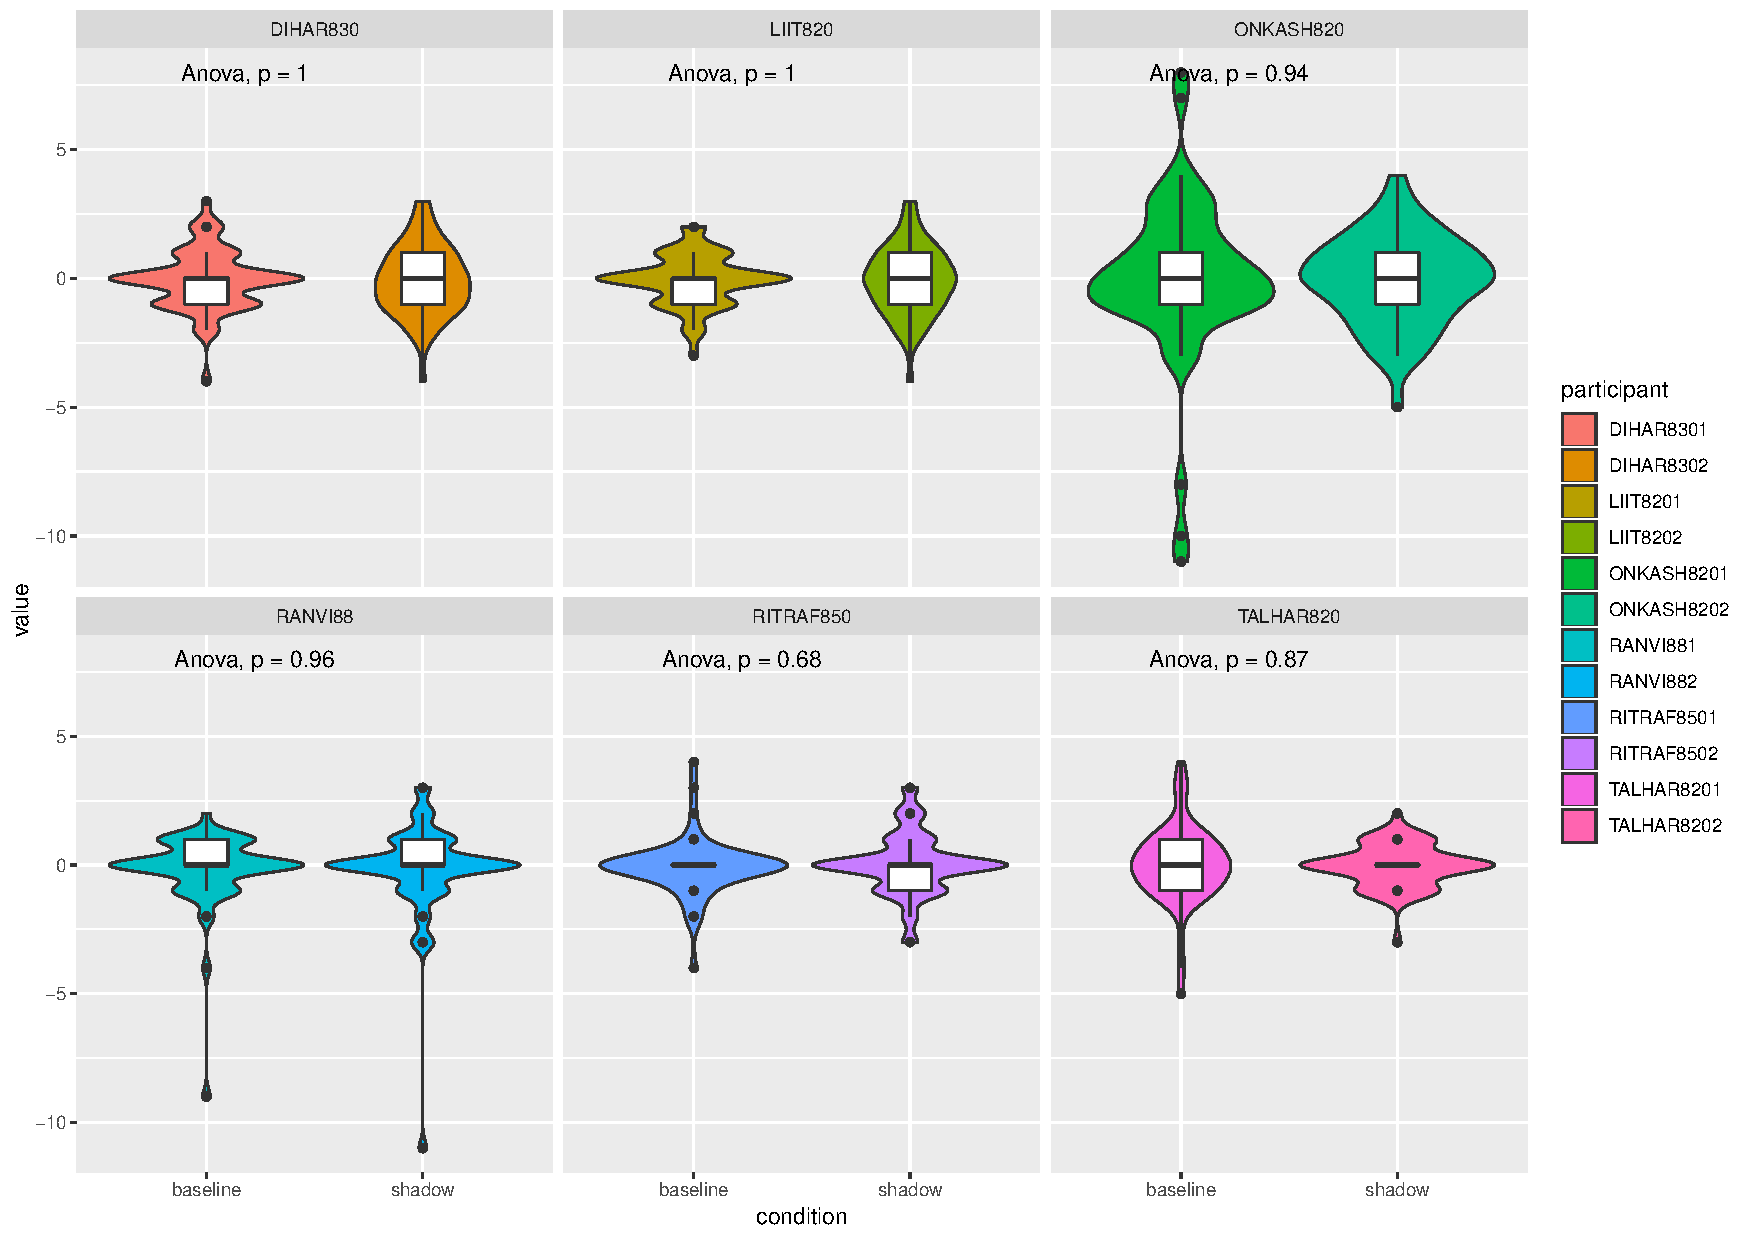
\includegraphics[width=\linewidth]{violin_facet_dev}
%	\caption{Comparison between the distribution of deviations from the correct intervals in baseline (red) and shadowing (blue) performances.
%		The numbers on the x-axis are the number of \acp{qt} above or below the correct interval.}
%	\label{fig:violin_facet_dev}
%\end{figure*}

\begin{table}
	\caption[Key and \acs{bpm} deviation summary]
			{Comparison between the singing tempo and key in baseline and shadowing performances of each participant.
			The values on the left and right under the key and \acs{bpm} columns are for baseline and shadowing performances, respectively.
			\acs{bpm}$\Delta$ shows the \acs{bpm} difference between baseline and shadowing, with the value in parentheses standing for the change in the difference from the recording's tempo.
			A negative value means that the participant decreased the distance to the recording.}
	\label{tab:bpm_and_keys}
	\centering
	\begin{tabularx}{\linewidth}{Xccc}
		\toprule
		\bfseries{Participant}	& \bfseries{Key}			& \bfseries{\acs{bpm}}		& \bfseries{\acs{bpm}$\Delta$}	\\
		\midrule
		RITRAF85				& F  |  F$\sharp$			& 76  |  70					&  6 ($-$6)						\\
		TALHAR82				& B  |  B$\flat$			& 57  |  63					&  6 ($-$2)						\\
		RANVI88					& A  |  A					& 59  |  63					&  4 (\phantom{$-$}0)			\\
		ONKASH82				& F$\sharp$  |  F$\sharp$	& 76  |  69					&  7 ($-$7)						\\
		LIIT82					& F$\sharp$  |  F$\sharp$	& 59  |  66					&  7 ($+$3)						\\
		DIHAR83					& F$\sharp$  |  F$\sharp$	& 62  |  61					&  1 ($-$1)						\\
		\rule{0pt}{0.5cm}% 
		recording				& B | (B)					& 61 | (61)					&								\\
		\bottomrule
	\end{tabularx}
\end{table}

In contrast to the first song, it was not expected that participants would be able to completely replicate all rhythmic elements in the second song.
Two participants managed to replicate part A (cf.\ \cref{snippet:uni-lullaby}), part B was replicated by three participants, and one participant replicated both part A and B.
The replication rate of each rhythmic element was measured separately instead of the overall tempo.
\cref{tab:neutral_rhythm_key} summarizes the occurrences of each rhythmic pattern R1--R4 (corresponding to the rhythmic patterns in bars 1, 9, 15, and 16 in \cref{snippet:uni-lullaby}, respectively) in the original and replicated versions.
The proportion of each pattern within a part was almost completely preserved in the replication, with the exception of a small difference between R2 and R3 in part A.
It is also evident that R1 and R4 were replicated more accurately.
An explanation for that is that they appear at the beginning and end of the song, making them easier to remember.
They are also technically easier to produce, since they contain fewer tones (and intervals) than R2 and R3.

The accuracy of tonal replication was measured in two ways, viz.\ directionality and quantity.
First, the correctness of the contour direction in each interval was evaluated (higher tone, lower tone, or same tone).
Second, the size of each interval was compared with the correct interval.
The participants correctly produced the contour direction in \SI{70}{\percent} of the intervals they replicated.
The intervals themselves, however, were correct only in \SI{44}{\percent} of the times.
This suggests that overall contours of the song are more easily recalled than the specific intervals.
\cref{snippet:deviation_example} shows a few specific examples of tonal and rhythmic deviations.

\section{Discussion and conclusion}
\label{sec:discussion_and_conclusion}

The experimental results presented in this paper show that convergence occurs in singing, more so with respect to temporal features than to tonal ones.
This stands in contrast to findings in interactive speech \citep[e.g.,][]{Raveh2019InterspeechAlexa}).
Even so, the results emphasize the similarity between the two oral capabilities, viz.\ speech and singing, which are both used in human communication.
They are therefore also prone to influence each other and can potentially be related and enhance one another.
For example, \citet[][p. 216]{Nardo2009musicality} explain that \emph{tonal} and \emph{rhythmic} abilities are measures of musicality and also related to phonetic talent.
This idea is also supported by \citet{Tsang2018musical}, who found a correlation between musical experience and sensitivity to convergence.
Similarly, pitch has been found to correlate with the level of agreement between interlocutors in dyadic conversation \citep{Okada2012interpreting}.
We therefore suggest that speech and music are two domains where certain common effects, and in particular convergence, occur with respect to shared prosodic features.
Establishing this connection between music and speech offers a wide variety of further interdisciplinary experimentation that combine linguistic and musical analysis methods.
Specifically for convergence, the influence of listening to people with different social and vocal characteristics can be examined.
The manner in which distances in vocal behavior decrease, or increase, can depend on further aspects of the social environment and auditory context, as suggested by \citet{Noy1999psychoanalysis}.

\begin{table}
	\caption[Percentages of rhythmic pattern replications]
		{Comparison between the percentage of occurrences of each rhythmic pattern in the original and replicated versions in all bar-level patterns.
		Parts A and B refer to the labels with the same letters in \cref{snippet:uni-lullaby}.
		Each replication row refers to the average over all participants who replicated that part.}
	\label{tab:neutral_rhythm_key}  
	\centering
	\begin{tabularx}{\linewidth}{XSSSS}
		\toprule
						& \bfseries{R1}		& \bfseries{R2}		& \bfseries{R3}		& \bfseries{R4}\\
		\midrule
		original part A	& 50				& 12.5				& 12.5				& 25\\
		replications A	& 54				& 18				& 7					& 21\\
		\rule{0pt}{0.5cm}%
		original part B	& 25				& 37.5				& 12.5				& 25\\
		replications B	& 25				& 42				& 8					& 25\\		
		\bottomrule
	\end{tabularx}
\end{table}

In conclusion, the first hypothesis -- convergence to perceived musical stimuli -- was satisfied, but not in the same way for pitch and tempo.
While tempo became globally closer to the recorded version in absolute terms, the tones were produced more precisely but within the same tonal range.
Additionally, the secondary expectation was only partially met, with fewer large deviations occurring in the shadowing performances, but otherwise the tones in the baseline production were slightly more accurate as a whole.
Finally, the third hypothesis was fulfilled, as the simpler, frequent rhythmic patterns were replicated more correctly.
Furthermore, with one exception, participants were not able to replicate the entire song.
%Interestingly, they remembered either part A or B, but didn't mix bars from both.

%\begin{figure}
%	\centering
%	\begin{subfigure}[t]{0.4\linewidth}
%	\centering
%	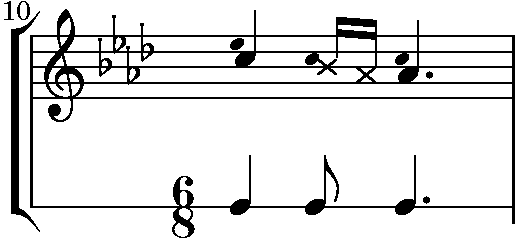
\includegraphics[width=\textwidth]{deviation_example_1}
%		\caption{Example 1}
%		\label{fig:deviation_example_1}
%	\end{subfigure}
%	\hfill
%	\begin{subfigure}[t]{0.6\linewidth}
%		\centering
%		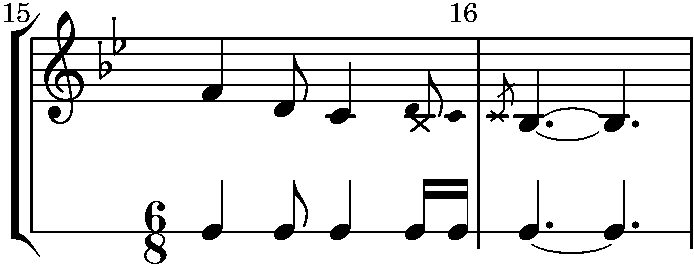
\includegraphics[width=\textwidth]{deviation_example_2}
%		\caption{Example 1}
%		\label{fig:deviation_example_2}
%	\end{subfigure}
%\end{figure}

\begin{snippet}[h]
	\centering
	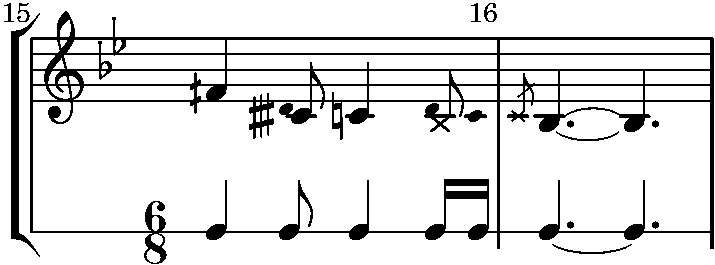
\includegraphics[width=0.9\linewidth]{deviation_example_2_mixed}
	\caption{Example of tonal (top staff) and rhythmic (bottom staff) deviations in the second lullaby.
			Smaller, stemless notes mark the correct notes where deviation occurred.
			Crossed-head notes mark those that deviate from the correct rhythmic pattern.}
	\label{snippet:deviation_example}
	\addcontentsline{lof}{section}{Snippet: example of tonal and rhythmic deviations}
\end{snippet}
